\fontfamily{\sfdefault}\selectfont
% XCircuit output "div_noise.tex" for LaTeX input from div_noise.ps
\def\putbox#1#2#3#4{\makebox[0.00000in][l]{\makebox[#1][l]{}\raisebox{\baselineskip}[0.00000in][0.00000in]{\raisebox{#2}[0.00000in][0.00000in]{\scalebox{#3}{#4}}}}}
\def\rightbox#1{\makebox[0.00000in][r]{#1}}
\def\centbox#1{\makebox[0.00000in]{#1}}
\def\topbox#1{\raisebox{-0.60\baselineskip}[0.00000in][0.00000in]{#1}}
\def\midbox#1{\raisebox{-0.20\baselineskip}[0.00000in][0.00000in]{#1}}
   \scalebox{1}{
   \normalsize
   \parbox{5.21354in}{
   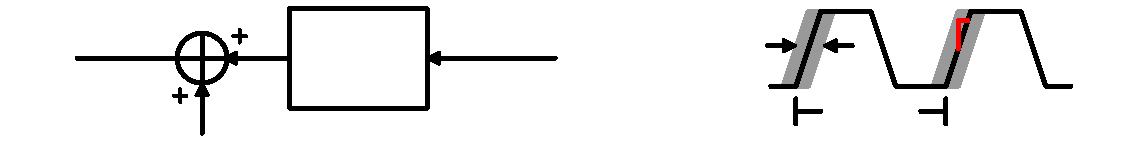
\includegraphics[scale=0.70000]{./figs/div_noise.pdf}\\
   % translate x=-72 y=528 scale 0.38
   \putbox{0.04200in}{0.55300in}{1.20}{$\Phi_{div}$[n]}%
   \putbox{2.06500in}{0.50400in}{1.20}{$\Phi_{out}$[n]}%
   \putbox{1.47000in}{0.40600in}{1.20}{$\div$ N}%
   \putbox{0.97300in}{0.05600in}{1.20}{$\Phi_{n_{div}}$}%
   \putbox{3.89200in}{0.16800in}{1.20}{$1/f_{ref}$}%
   \putbox{3.40900in}{0.58100in}{1.20}{$\sigma_{\Phi n_{div}}$}%
   \putbox{4.25600in}{0.56700in}{1.20}{$\frac{dV}{dt}$}%
   } % close 'parbox'
   } % close 'scalebox'
   \vspace{-\baselineskip} % this is not necessary, but looks better
\fontfamily{\rmdefault}\selectfont
